% Supplementary material for the PVLDB 2027 submission.
% Compile with: pdflatex supplementary.tex
\documentclass[sigconf, nonacm]{acmart}

%%% do not modify the following VLDB block %%%
\usepackage{pvldb}
%%% VLDB block end %%%
\usepackage{array}
\usepackage{tabularx}
\raggedbottom
\vfuzz=3pt

\renewcommand\vldbdoi{XX.XX/XXX.XX}
\renewcommand\vldbpages{XXX-XXX}
\renewcommand\vldbavailabilityurl{}

\begin{document}
\title{Supplementary Material for\\When Execution Evidence Is Incomplete: Measuring and Repairing Observability in Value-Level Data Lineage}

\author{Xu Gao}
\affiliation{\institution{Zhejiang University}\country{China}}
\email{gx\_zjumail@zju.edu.cn}

\author{Sai Wu}
\affiliation{\institution{Zhejiang University}\country{China}}
\email{wusai@zju.edu.cn}

\author{Xiu Tang}
\affiliation{\institution{Zhejiang University}\country{China}}
\email{tangxiu@zju.edu.cn}
\thanks{Xiu Tang and Chang Yao are the corresponding authors.}

\author{Chang Yao}
\affiliation{\institution{Zhejiang University}\country{China}}
\email{changy@zju.edu.cn}

\author{Gang Chen}
\affiliation{\institution{Zhejiang University}\country{China}}
\email{cg@zju.edu.cn}

\maketitle

\appendix
\section{Artifact Layout}
\label{app:artifact}

The artifact contains the 30-query gold sheet and arbitration log, the 170-query silver predictions, the strict split files, the literal ablation, the dbt seed data, and the scripts that regenerate every table. The paper/ directory contains the \LaTeX{} source and figures; results/ contains per-query predictions and metrics; data/ contains query sets and dbt seeds; src/agentdb/ contains the oracle, lineage, metrics, and evolution code; scripts/ contains the experiment drivers. The strict split is deterministic (pre-specified seed and SQL-template grouping), and the raw per-query predictions are included so that the negative result can be audited independently.

\section{Annotation Protocol Details}
\label{app:annotation}

\begin{table}[t]
\centering
\small
\caption{Annotation protocol summary.}
\label{tab:annprotocol}
\begin{tabular}{ll}
\toprule
Item & Value \\
\midrule
Queries & 30 (6 per category) \\
Annotators & 3 independent \\
Calibration & 5 joint queries \\
Labeling & blind, then compare, then merge \\
Arbitration & third annotator \\
Final gold & 87 pos / 2 neg / 7 unk \\
Agreement & pairwise binary $\kappa=0.942$--$1.000$ \\
\bottomrule
\end{tabular}
\end{table}

The 30 queries were sampled across eight Spider databases; the six-per-category design ensures that projection, join, aggregate, CTE, and CASE are represented. The unknown edges are caused by anonymized values or type mismatches in the local instance, not by annotator disagreement.

\section{Split Construction Details}
\label{app:split}

\begin{table}[t]
\centering
\small
\caption{Split construction counts.}
\label{tab:splitsrc}
\begin{tabular}{lcc}
\toprule
Step & Removed & Remaining \\
\midrule
Main queries & -- & 130 \\
Gold subset & 30 & 100 non-gold \\
Gold SQL template overlap & 22 & 78 strict pool \\
Strict split & -- & 43 / 16 / 19 \\
Stress queries & -- & 40 \\
Unique pool & -- & 170 \\
\bottomrule
\end{tabular}
\end{table}

\begin{table}[t]
\centering
\small
\caption{Pilot and strict split counts. Pilot gold queries overlap policy training; strict excludes gold queries and identical SQL templates.}
\label{tab:split}
\begin{tabular}{lcccc}
\toprule
Split & Pilot n & Pilot gold & Strict n & Strict gold \\
\midrule
Train & 65 & 30 & 43 & 0 \\
Validation & 26 & 0 & 16 & 0 \\
Test & 18 & 0 & -- & -- \\
Regression & 21 & 0 & 19 & 0 \\
Gold (evaluation) & -- & 30 & 30 & 30 \\
\bottomrule
\end{tabular}
\end{table}

The 22 removed queries are not discarded: they remain in the 170-query calibrated-reference evaluation and in the main coverage analysis, but they do not participate in policy learning.

\section{Representative Queries}
\label{app:examples}

\begin{verbatim}
SELECT Name FROM singer WHERE Country = 'France';
\end{verbatim}
The static parser reports \texttt{Country} as a syntactic reference. The execution oracle witnesses the control edge only if a row can be made to satisfy the predicate; the literal probe uses \texttt{'France'} from the query, while an arbitrary cell value does not.

\begin{verbatim}
SELECT count(*) FROM concert
WHERE Year = 2014 OR Year = 2015;
\end{verbatim}
A larger budget with the same arbitrary values does not help; the literal probe tries 2014 and 2015 and changes the count from 0 to 1.

\begin{verbatim}
SELECT c.country, SUM(o.amount) AS revenue
FROM {{ ref('stg_orders') }} o
JOIN {{ ref('stg_customers') }} c
  ON o.customer_id = c.customer_id
GROUP BY c.country
\end{verbatim}
The raw template fails to parse; after Jinja expansion, static lineage parses but misses control edges. The oracle recovers them, and literal probing recovers most of them at a lower cost than an exhaustive reference.

\section{Additional Results}
\label{app:extra}

Figure~\ref{fig:fn} breaks down the 11 positive edges missed by the machine reference on the human-gold set. Ten of the 11 involve predicate or control clauses: six WHERE-filter columns, two CASE-derived outputs, and two GROUP BY keys; one is a coercion-only join. The clause labels are descriptive and come from the human audit, not from a semantic ground-truth taxonomy. This anatomy is the reason literal probing is targeted at predicates rather than at more cell values.

\begin{figure}[t]
\centering
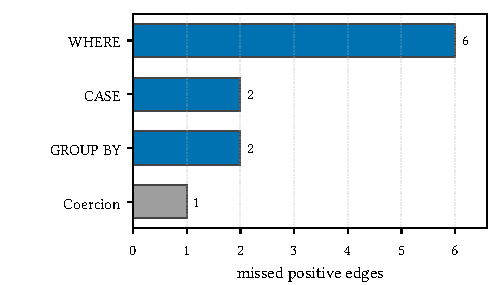
\includegraphics[width=\columnwidth]{figures/fn_anatomy.pdf}
\caption{Anatomy of the machine reference's 11 missed positive edges on the 30-query human gold. Ten involve predicate or control clauses; one is a coercion-only join. Counts come from the human audit.}
\label{fig:fn}
\end{figure}

Table~\ref{tab:nongold} reports the non-gold check discussed in Section~3.5 of the main paper. The 100 queries are the main queries that remain after removing the 30 human-gold queries. They are evaluated against the machine reference, not against human labels; an edge predicted outside the reference is therefore unjudged rather than known to be wrong. We count such edges as false positives, which makes the reported precision a conservative lower bound. Literal probing alone is more precise but lower-coverage than the Static+Cell baseline. The union recovers the coverage lost by either method alone: coverage rises from 0.694 to 0.822, precision falls from 0.888 to 0.844, and F1 rises from 0.779 to 0.833. Because the reference shares the predicate blind spot documented in Section~3.2 of the main paper, these numbers measure agreement and coverage, not independent accuracy.

\begin{table}[h!]
\centering
\small
\caption{100 non-gold queries against the machine reference.}
\label{tab:nongold}
\begin{tabular}{lccc}
\toprule
Method & Precision & Coverage & F1 \\
\midrule
Static+Cell & 0.888 & 0.694 & 0.779 \\
Literal & 0.905 & 0.640 & 0.750 \\
Static+Literal & 0.844 & 0.822 & 0.833 \\
\bottomrule
\end{tabular}
\end{table}

Table~\ref{tab:splithalf} repeats the literal comparison on two pre-specified halves of the 30 gold queries. Both halves show a positive literal margin: F1 rises from 0.773 to 0.875 ($+0.102$) in the first half and from 0.681 to 0.723 ($+0.042$) in the second. The Lit$\,\cup\,$Evo row is higher in both halves, but it contains literal probing, so it does not separate the contribution of evolution from the contribution of literal probing. The split is a stability check on a 30-query discovery set, not an independent confirmation set, and the halves are not used to tune any policy.

\begin{table}[h!]
\centering
\small
\caption{Split-half stability on the 30 gold queries.}
\label{tab:splithalf}
\begin{tabular}{lccc}
\toprule
Method & First-15 F1 & Second-15 F1 \\
\midrule
Static+Cell & 0.773 & 0.681 \\
Literal & 0.875 & 0.723 \\
Literal$\cup$evolving & 0.941 & 0.824 \\
\bottomrule
\end{tabular}
\end{table}

Table~\ref{tab:transition} isolates the mechanism at the edge level. Literal probing is not a superset of Static+Cell: it recovers 17 control edges but loses 10 edges (9 DATA and 1 MIXED), so the union is the appropriate predictor. It introduces no false positives on the two gold-negative edges. This is also why the paper reports the union rather than literal probing alone.





\begin{table}[h!]
\centering
\small
\caption{Edge-level transitions from Static+Cell (S+C) to literal probing on the 30 gold queries (87 positive edges, 2 negative edges).}
\label{tab:transition}
\begin{tabular}{llc}
\toprule
S+C & Literal & Edges \\
\midrule
TP & TP & 38 \\
FN & TP & 17 (all CONTROL) \\
TP & FN & 10 (9 DATA, 1 MIXED) \\
FN & FN & 22 \\
TN & TN & 2 \\
\bottomrule
\end{tabular}
\end{table}

\section{Experiment Commands}
\label{app:commands}

The commands assume execution from the repository root and Python 3.11 or newer. Install the package and the optional dependencies used by the dbt and figure scripts:
\begin{verbatim}
pip install -e .
pip install jinja2 matplotlib
\end{verbatim}
The scripts read the Spider SQLite databases from the default database directory; pass \texttt{--db-dir} to override this path. The order below builds the query sets first, then the coverage, human-gold, held-out, silver, ablation, and dbt results. The statistics scripts consume those JSON files, and the figure script consumes the statistics and per-query outputs.

\begin{verbatim}
python scripts/build_query_sets.py
python scripts/run_p1_coverage.py
python scripts/evaluate_gold.py
python scripts/heldout_gold.py
python scripts/evaluate_silver.py
python scripts/evaluate_nongold.py
python scripts/literal_ablation.py
python scripts/run_p3_dbt_ext.py
python scripts/compute_stats.py
python scripts/gold_stats.py
python scripts/classify_gold_edges.py
python paper/figures/make_all_figures.py
\end{verbatim}

Each experiment writes JSON under \texttt{results/}; the figure script writes the nine PDFs under \texttt{paper/figures/}. The oracle opens a SQLite savepoint before each perturbation and rolls it back afterward, so the seed databases are not modified. Query order and split files are deterministic; randomized components such as candidate sampling and the paired bootstrap use deterministic seeds (42) in the scripts. The new three-state, external-control, and scale results are regenerated by the four new scripts in \texttt{scripts/}; the scale and ProvSQL runs require the SF0.1 SQLite export and a ProvSQL-enabled PostgreSQL instance, respectively.

\clearpage
\section{Additional Tables}

The following tables were moved out of the main paper to keep the body within the 12-page limit. They are reproduced here without changing their content.

\begin{center}
\captionof{table}{Policy search space (per SQL category).}
\label{tab:policy}
\begin{tabular}{lc}
\toprule
Dimension & Values \\
\midrule
Row budget & 1, 3, 5, 10 \\
Families & \{cell\}, \{cell, null families\} \\
Selection & validation F1, tie-break cost \\
Acceptance & no regression $>$ 2 pp \\
Training queries & 43 (strict) \\
\bottomrule
\end{tabular}
\end{center}

\begin{center}
\captionof{table}{Failure taxonomy of unobserved control edges.}
\label{tab:taxonomy}
\small
\begin{tabular}{lll}
\toprule
Cause & Example & Status \\
\midrule
Predicate literal & WHERE Country='France' & literal probe \\
Threshold literal & WHERE Year=2014 & literal probe \\
CASE boundary & AVG(capacity)>0 & boundary probe \\
Coercion & TEXT vs numeric ID & open \\
Multi-condition & two predicates & open \\
LIMIT/fan-out & unselected rows & abstain \\
\bottomrule
\end{tabular}
\end{center}

\begin{center}
\captionof{table}{Evaluation settings.}
\label{tab:settings}
\small
\begin{tabular}{ll}
\toprule
Item & Setting \\
\midrule
Queries & 130 main, 40 stress, 30 gold \\
Annotation & 3 annotators, mean pairwise binary $\kappa=0.961$ \\
Strict split & 43 train, 16 val, 19 regression \\
Primary metric & macro query-level F1 \\
Secondary & micro F1, recall, cost \\
Statistics & paired bootstrap, BH-FDR \\
Cost unit & mean executions per query (total = 30$\times$mean) \\
\bottomrule
\end{tabular}
\end{center}

\begin{center}
\scriptsize
\setlength{\tabcolsep}{2pt}
\captionof{table}{Blind-spot and transition replication. C=CONTROL, D=DATA, M=MIXED.}
\label{tab:replication}
\begin{tabular}{lcc}
\toprule
Statistic & Discovery & Confirmation \\
\midrule
Positive edges & 87 & 145 \\
Machine misses & 11 & 18 \\
CONTROL/MIXED misses & 10 & 18 \\
DATA misses & 1 & 0 \\
FN$\to$TP & 17 (all CONTROL) & 22 (20 C, 2 M) \\
TP$\to$FN & 10 (9 D, 1 M) & 25 (21 D, 3 M, 1 C) \\
\bottomrule
\end{tabular}
\end{center}

\begin{center}
\captionof{table}{Confirmation macro F1 by SQL category.}
\label{tab:conf-category}
\begin{tabular}{lccc}
\toprule
Category & Static+Cell & Literal & Union \\
\midrule
Projection & 0.815 & 0.792 & 0.933 \\
Join & 0.729 & 0.773 & 0.851 \\
Aggregate & 0.750 & 0.824 & 0.857 \\
CTE & 0.880 & 0.833 & 0.963 \\
CASE & 0.792 & 0.684 & 0.840 \\
\bottomrule
\end{tabular}
\end{center}

\begin{center}
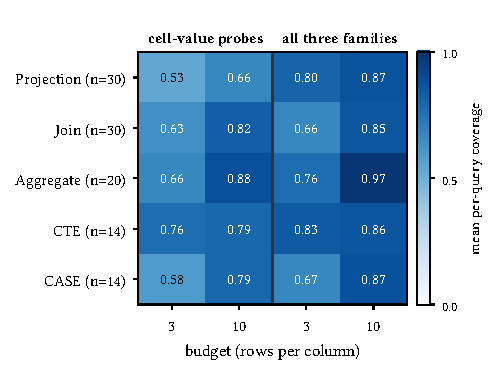
\includegraphics[width=\columnwidth]{figures/heatmap.pdf}
\captionof{figure}{Coverage on the 108 main queries with at least one reference edge. Each cell is the mean per-query fraction of reference edges recovered; $n$ is the number of queries in the SQL category. The first two columns perturb cell values only; the last two add value-to-null and null-to-value. The color scale spans 0--1 without clipping.}
\label{fig:heatmap-supp}
\end{center}

\begin{center}
\captionof{table}{Real-value TPC-H control: 6k (SF0.001), 60k (SF0.01), and 600k (SF0.1) lineitem rows; 8 hand-specified control edges.}
\label{tab:tpch-control}
\begin{tabular}{lccc}
\toprule
Method & 6k rows & 60k rows & 600k rows \\
\midrule
Cell-only (b=3) & 2/8 & 2/8 & 2/8 \\
LineageX (static) & 6/8 & -- & -- \\
Literal (b=3) & 7/8 & 7/8 & 7/8 \\
\bottomrule
\end{tabular}
\end{center}

At 600k rows, mean wall-clock is 7.0 s for cell-only and 52.6 s for literal probing per query (on-disk SQLite); the 60k control measured 0.44 s and 2.7 s.

\begin{center}
\captionof{table}{Control/DATA complement on the six TPC-H control queries. ProvSQL q4 aggregate where-provenance is unsupported, so its DATA denominator is 7; this is a control-focused comparison, not a full lineage benchmark.}
\label{tab:tpch-external}
\begin{tabular}{lcc}
\toprule
Method & CONTROL (8) & DATA (7) \\
\midrule
Static (sqlglot) & 0 & 7 \\
ProvSQL where-provenance & 0 & 6 \\
Cell-only (b=3) & 2 & 5 \\
Literal (b=3) & 7 & 5 \\
Static+Literal & 7 & 7 \\
\bottomrule
\end{tabular}
\end{center}

Table~\ref{tab:tristate} evaluates the operational oracle on the 42-template confirmation gold. It returns \textsc{Positive} for 137/145 confirmed positives and \textsc{Negative} for 184/313 confirmed negatives, with no inversion of a confirmed edge; 6 additional \textsc{Negative} outputs are human-unknown. The 129 negative edges left \textsc{Unknown} are those covered by the incompleteness guards; the 8 positive edges left \textsc{Unknown} are grouped or subquery cases.

\begin{center}
\begin{minipage}{\linewidth}
\centering
\captionof{table}{Operational three-state oracle on the 42-template confirmation gold (492 edges). Columns are human labels; rows are oracle states. \textsc{Negative} is relative to the declared 30-row snapshot and candidate space.}
\label{tab:tristate}
\begin{tabular}{lccc}
\toprule
Oracle state & Human POS & Human NEG & Human UNK \\
\midrule
\textsc{Positive} & 137 & 0 & 0 \\
\textsc{Negative} & 0 & 184 & 6 \\
\textsc{Unknown} & 8 & 129 & 28 \\
\bottomrule
\end{tabular}
\end{minipage}
\end{center}

\begin{center}
\captionof{table}{Bootstrap 95\% CIs for macro F1 (10,000 resamples, seed 42).}
\label{tab:ci}
\begin{tabular}{llc}
\toprule
Set & Method & Macro F1 [95\% CI] \\
\midrule
Discovery & Static+Cell & 0.574 [0.426, 0.715] \\
Discovery & Literal & 0.728 [0.600, 0.842] \\
Confirmation & Static+Cell & 0.704 [0.595, 0.803] \\
Confirmation & Literal & 0.723 [0.631, 0.808] \\
Confirmation & Static+Literal & 0.819 [0.729, 0.897] \\
\bottomrule
\end{tabular}
\end{center}

\begin{center}
\begin{minipage}{\linewidth}
\centering
\captionof{table}{Positioning relative to closest work.}
\label{tab:positioning}
\begin{tabularx}{\linewidth}{>{\raggedright\arraybackslash}p{2.75cm}>{\raggedright\arraybackslash}X}
\toprule
Work & Focus \\
\midrule
LineageX & parse-tree SQL column lineage \\
Smoke/SAC & execution/provenance lineage \\
SLiCE & multilingual pipeline lineage \\
LLM lineage & catalog-based reconstruction \\
AgentDevel/VERSE & agent harness, execution feedback \\
Agent-Sentry & execution provenance for agent bounds \\
This work & differential execution + literals \\
\bottomrule
\end{tabularx}
\end{minipage}
\end{center}

\paragraph{Evidence map.}
\begin{itemize}
\item \textbf{30-query gold.} Supports observability-gap analysis and method design; does not support confirmatory accuracy or an independent test.
\item \textbf{42-template confirmation.} Supports post-freeze confirmation of Literal and Static+Cell; does not support evolution independence or an external benchmark.
\item \textbf{170-query silver.} Supports agreement, coverage, and cost at scale; does not support independent gold accuracy or universal recall.
\item \textbf{30 dbt/Jinja cases.} Supports a heterogeneous SQL pipeline case study and macro expansion; does not support full dbt-runtime or production behavior.
\item \textbf{6 TPC-H controls.} Supports real-value, scale-oriented control and blind-spot persistence; does not support a production benchmark or general accuracy.
\end{itemize}

\section{Limitations and Threats to Validity}
\label{app:limitations}

\emph{Construct validity.} We operationalize value lineage as instance-level
counterfactual influence under a declared perturbation family. This is measurable
and reproducible, but it is not universal semantic dependency; a different
family could change the edge set. We report the family explicitly and treat it
as part of the claim.

\emph{Internal validity.} The strict split removes gold queries and identical
SQL templates, but it cannot remove all distributional overlap between train and
gold. The pilot-to-strict change removes query overlap, template overlap, and the
22 removed queries together, so we do not attribute the difference to one factor
alone. The learned policy is small and the validation set is small; a larger
policy space could behave differently. The negative result is specific to the
evaluated policy space and split protocol.

\emph{External validity.} Spider is a cross-domain benchmark; our main instance
is anonymized and the queries are not production pipelines. The TPC-H control
now includes SF0.1 with 600,572 lineitem rows, but it remains one benchmark
schema; we treat it as scale-oriented controlled validation, not production
validation. The dbt/Jinja cases are simulated with Jinja2, not a full dbt runtime,
and serve as a heterogeneous SQL pipeline case study. The main experiments use
SQLite affinity; dynamic SQL, UDFs, and stored procedures are outside scope.
The results may not transfer to production warehouses with materialization,
incremental models, or warehouse-specific SQL. LineageX is run without a
database connection as an external static baseline. ProvSQL where-provenance is
run on the six TPC-H control queries (Table~\ref{tab:tpch-external}); we could
not locate a public artifact for Smoke or SAC that supports a head-to-head run.
The sqlglot baseline is evaluated separately on DATA and CONTROL edges.

\emph{Statistical validity.} The discovery gold set has 30 queries, the
human-gold confirmation set 42, and the strict training set 43. Confidence
intervals are wide, and some comparisons are borderline. We report paired
bootstrap intervals and avoid claiming significance where the interval crosses
zero. On the confirmation set, literal probing alone is not significant; the
union is.

\end{document}
